\subsection{Bluetooth}\label{sec:bluetooth}


\subsubsection{Major Minor Vergabe}
Um die Major Minor Nummern mit dem Dojo zu benutzen wurden sie im Verlaufe des Projektes Standartisiert. Es sind Bereiche definiert für die speziellen Funktionen der Software. Die Sprachauswahl fuktioniert über solche Nummern. Beacons mit diesen Speziellen Nummeren lösen auf dem Dojo entsprechende Funktionen aus. Auf Abbildung \ref{fig:Bluetooth_def_MM} sind die ersten Definitionen beschrieben. Die Nummerenräume sind so gestaltet, dass es genug Platz hat, um zusätzliche Funktionen hizuzufügen, zum Beispiel weitere Sprachen oder Zugangskontrollen.

\begin{figure}[htbp!!!!]
	\centering
	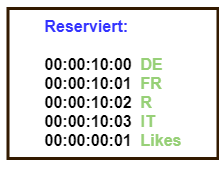
\includegraphics[width=0.5\textwidth]{Data/Reserviert_picture.png}
	\caption[Software:Definierte MM]{Default Definitionen von speziellen Major Minor Nummern.}
	\label{fig:Bluetooth_def_MM}
\end{figure}

In Abbildung \ref{fig:Bluetooth_MM_Vergabe} ist zu sehen, dass die erste Major Nummer 0x00 sein muss damit ein spezieller Beacon erkennt wird. Das vereinfacht das Programm, da bei einem neuen Ble-Package nur der erste Eintrag im Array betrachtet werden muss, um die speziellen Beacons zu erkennen. Der Nummernraum für spezielle Beacons umfasst ca 16 Mio. Adressen, was für zusätzliche Funktionen reichen sollte. Sommit bleiben ca 4.2 Mia. Adressen für Kunstwerke übrig.


\begin{figure}[htbp!!!!]
	\centering
	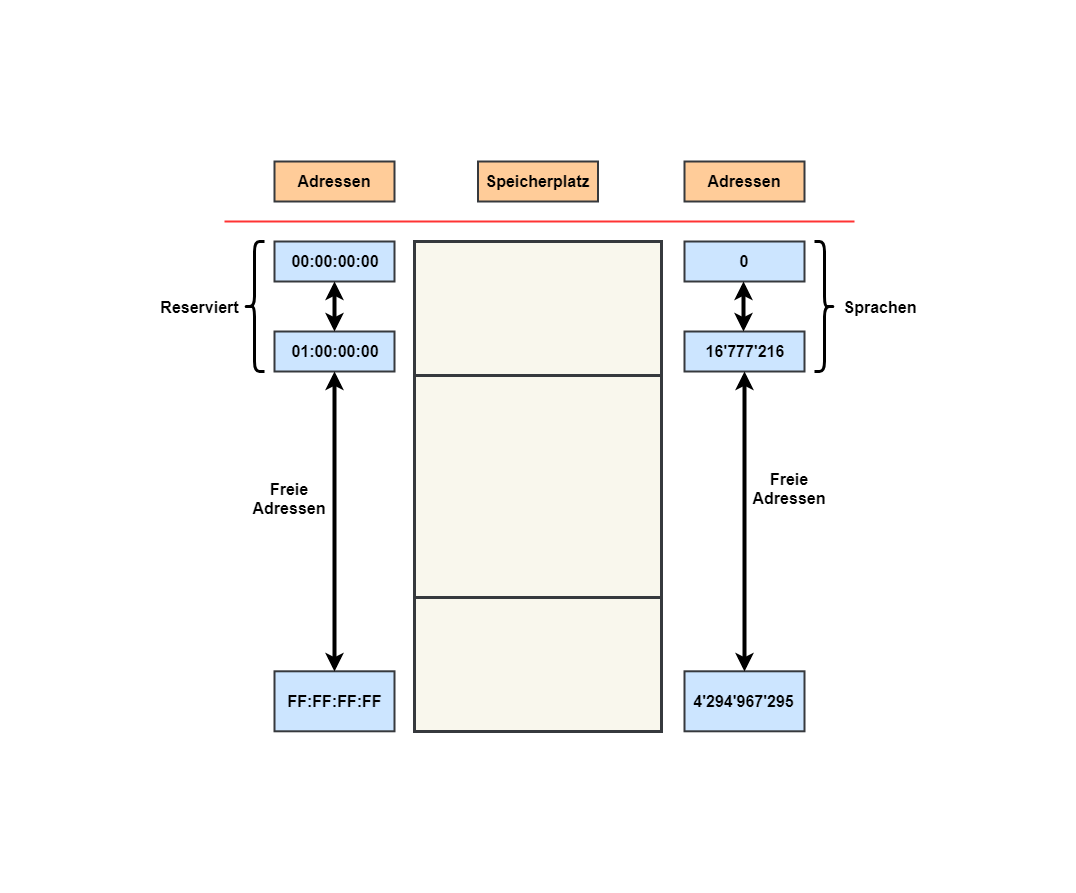
\includegraphics[width=0.7\textwidth]{Data/Speicheradressen_picture.png}
	\caption[Software:MM Vergabe]{Definition der Majo Minor Vergabe}
	\label{fig:Bluetooth_MM_Vergabe}
\end{figure}



